\documentclass[onecolumn, draftclsnofoot,10pt, compsoc]{IEEEtran}

\usepackage{graphicx}
\usepackage{url}
\usepackage{setspace}
\usepackage{geometry}
\usepackage{listings}
\usepackage{color}
\usepackage{etoolbox}
\usepackage{pdflscape}


\geometry{textheight=9.5in, textwidth=7in}

% 1. Fill in these details
\def \CapstoneTeamName{			              			 PlanteR-GB}
\def \CapstoneTeamNumber{					           			 Group 64}
\def \GroupMemberOne{				           				Austin Hodgin}
\def \GroupMemberTwo{				           				Travis Hodgin}
\def \GroupMemberThree{			            Maximillian Schmidt}
\def \GroupMemberFour{		        	             Zach Lerew}
\def \CapstoneProjectName{	      	    Winter is Coming...}
\def \CapstoneSponsorCompany{		    Oregon State University}
\def \CapstoneSponsorPerson{		 			  				 Victor Hsu}

% 2. Uncomment the appropriate line below so that the document type works
\def \DocType{		%Problem Statement
				%Requirements Document
				Technology Review
				%Design Document
				%Progress Report
				}

\newcommand{\NameSigPair}[1]{\par
\makebox[2.75in][r]{#1} \hfil 	\makebox[3.25in]{\makebox[2.25in]{\hrulefill} \hfill		\makebox[.75in]{\hrulefill}}
\par\vspace{-12pt} \textit{\tiny\noindent
\makebox[2.75in]{} \hfil		\makebox[3.25in]{\makebox[2.25in][r]{Signature} \hfill	\makebox[.75in][r]{Date}}}}
% 3. If the document is not to be signed, uncomment the RENEWcommand below
\renewcommand{\NameSigPair}[1]{#1}

%%%%%%%%%%%%%%%%%%%%%%%%%%%%%%%%%%%%%%%
\begin{document}
\begin{titlepage}
    \pagenumbering{gobble}
    \begin{singlespace}
    	%\includegraphics[height=4cm]{coe_v_spot1}
        \hfill

        % 4. If you have a logo, use this includegraphics command to put it on the coversheet.
        %
\includegraphics[height=4cm]{derp.jpg}

        \par\vspace{.2in}
        \centering
        \scshape{
            \huge CS Capstone \DocType \par
            {\large\today}\par
            \vspace{.5in}
            \textbf{\Huge\CapstoneProjectName}\par

            %\vfill
						\vspace{1in}

            {\large Prepared for}\par
            \Huge \CapstoneSponsorCompany\par
            \vspace{5pt}
            {\Large\NameSigPair{\CapstoneSponsorPerson}\par}

						\vspace{1in}

            {\large Prepared by}\par
						{\huge \CapstoneTeamNumber}\par
            \CapstoneTeamName\par
            \vspace{5pt}

            {
							\Large
							%\NameSigPair{\GroupMemberOne}\par
							%\NameSigPair{\GroupMemberTwo}\par
							%\NameSigPair{\GroupMemberThree}\par
							\NameSigPair{\GroupMemberFour}\par
            }

            \vspace{20pt}
        }

				\newpage
        \begin{abstract}
				\noindent The Control Service is a crucial piece of this system. It receives incoming data from client interfaces, processes and stores it, and then sends it to the LED control system.
				This system will have multiple clients, and possibly multiple LED controllers. The singular path between those two groups is the Control Service, making it a bottleneck of the system.
				The technology used for the inlet, processing, and outlet of the Control Service will determine the overall throughput of the system.
				This document will compare three technologies for the processing of client input, the internal representation of data, and the storage of system parameters for persistence.
        \end{abstract}
    \end{singlespace}
\end{titlepage}

\newpage

\pagenumbering{arabic}
\tableofcontents
% 7. uncomment this (if applicable). Consider adding a page break.
%\listoffigures
%\listoftables
\clearpage
\singlespace

\newpage


% Syntax highlighting
\definecolor{mygreen}{rgb}{0,0.6,0}
\definecolor{mygray}{rgb}{0.5,0.5,0.5}
\definecolor{mymauve}{rgb}{0.58,0,0.82}

\lstset{
  backgroundcolor=\color{white},   % choose the background color
  basicstyle=\footnotesize,        % size of fonts used for the code
  breaklines=true,                 % automatic line breaking only at whitespace
  captionpos=b,                    % sets the caption-position to bottom
  commentstyle=\color{mygreen},    % comment style
  escapeinside={\%*}{*)},          % if you want to add LTeX within your code
  keywordstyle=\color{blue},       % keyword style
  stringstyle=\color{mymauve},     % string literal style
	frame = single,                  % code framing
}


	% Document body
		%Purpose of tech, derived from tech, example usage, projects that use.
		%Critical thinking, research, comparison to other tech
	\section{Control Service API}
		\subsection{Overview and Criteria}
		The control service is the bridge between the user interface and the LEDs.
		The API (application programming interface) will serve as the entry point for all changes made to the system.
		The method with which the UI and the control service communicate is obfuscated from the user, but is an important factor in the speed and reliability of the system.
		The control service interface needs to be versatile enough to support the rapid addition of new features, and simple enough that it does not become a bottleneck in the system.

		\subsubsection{REST}
		REST stands for \textbf{Re}presentational \textbf{S}tate \textbf{T}ransfer.
		It is an architectural style and modern approach to web service communication. \cite[ch.5]{rest1}
		REST provides a lightweight communication protocol between client and server,
		making it a popular building style for cloud-based APIs.
		It is used commonly all over the web, and by companies like Amazon, Microsoft, and Google. \cite{rest2}
		The architecture provides a limited set of actions (verbs) which accompany each request and determine how the data is processed: GET, POST, PUT, and DELETE.
		Flexibility is provided by assigning resources (nouns) to a specific URL.
		REST applications typically send data over HTTP, which can be parsed by existing web technologies, meaning it can be displayed or analyzed in a web page easily.

		\noindent \\In the context of this system, a request to a REST driven Control Service could look like this:
		\begin{lstlisting}[language=XML]
POST http://localhost:5324/api/update/zone/
Host: localhost
Content-Type: text/xml; charset=utf-8
Content-Length: 123
<?xml version="1.0" encoding="utf-8"?>
<Zone>
  <ID>3</ID>
  <Color>RED</Color>
  <Intensity>40</Intensity>
  <PwrState>On</PwrState>
</Zone>
		\end{lstlisting}


		\noindent \\The control flow of the Control Service with a REST API may look like this:

		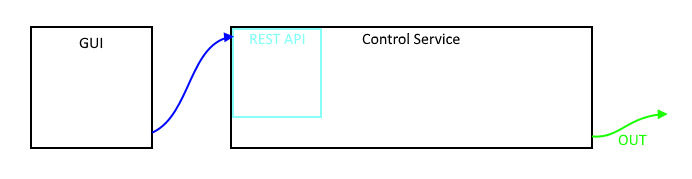
\includegraphics[width=\linewidth]{RESTDiag.png}

		\noindent \\Advantages of using REST architecture:
		\begin{itemize}
			\item Adding new data manipulation routes is simple and fast, simply bind a route (\textit{/api/update/schedule/}) to a function (\textit{void UpdateSchedule(request)})
			\item Control Service and interface are separated and do not need to understand each other's inner structure to transfer data
			\item Control Service can assume the role of the \textit{server} in the client-server model by responding to client requests, removing the need for a nodeJS web server to take in requests
			\item Control Service can respond to local network requests with no extra effort, allowing the GUI to be hosted on a different networked device (distributed systems)
		\end{itemize}

		\noindent \\Disadvantages of using a REST architecture:
		\begin{itemize}
			\item Language support is mostly ubiquitous, but some library implementations may be better than others
			\item HTTP may have some minor overhead
		\end{itemize}

		%GUI (Makes changes and sends cross-origin input to REST API) ->
		%Control service (Listens for CRUD requests, ex:localhost:8324/api/edit/zone/1/color/red) ->
		%Control service (Updates internal system state and writes to config file for persistence) ->
		%Control service (Gets submit request, )
		%Control service - Pull changes from config file, and incorporate changes into driving language file ->
		%Upon _localhost:8324/api/submit_ - Control service - Recompile driving language file, do something with the hex

		\subsubsection{File manipulation}
		File manipulation is a method of communication where the web server and Control Service communicate through the direct modification of a shared configuration file.
		This system works by having a standard configuration file structure which is known by both the web server and control service.
		System settings are changed in the client interface and posted to the web server, which opens and modifies the configuration file it shares with the control service.
		The Control Service monitors the configuration file for changes, and reloads its internal state when changes are detected.
		There are several options for configuration files, such as XML, JSON, or YAML. \cite{config1}
		Using this option would leverage the Unix file system for data transfer between web server and control service.

		\noindent \\In this system, the control flow for a file manipulation interface may look like this:

		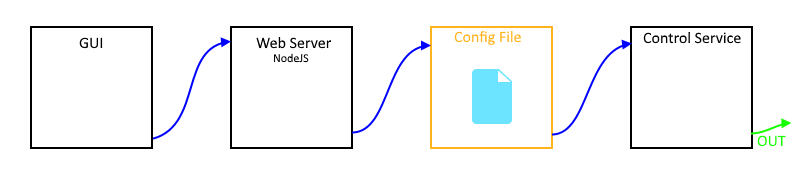
\includegraphics[width=\linewidth]{FileManipDiag.png}

		\noindent \\Advantages of using file manipulation:
		\begin{itemize}
			\item Persistent storage would come automatically
		\end{itemize}

		\noindent \\Disadvantages of using file manipulation:
		\begin{itemize}
			\item File I/O is very time consuming, and requires the entire file to be read each time a change is made
			\item The web server and control service both need to read and write to the configuration file, requiring the maintenance of two parsing functions in different languages to be maintained
			\item File manipulation must be synchronous - the system cannot read and write to the file at the same time
		\end{itemize}

		%GUI - Front end client makes changes ->
		%GUI - Javascript back end of some sort that takes client requests and reads (parses) config file, writes changes
		%Control service -> Reads changes to config file (parses), update internal state ->
		%Control service -> Applies changes through GPIO or recompile HEX

		\subsubsection{Socket IPC}
		Socket IPC (inter-process communication) is a method of communication where the web server and Control Service communicate through a socket connection.
		Socket communication works by establishing a communication link between a client and the server, which remains open for the duration of the transaction. \cite{socket1}
		Once data is transferred, the socket is closed. Sockets can communicate between devices on a local network, or between processes on a single device.


		\noindent \\In this system, the control flow for a socket IPC interface may look like this:

		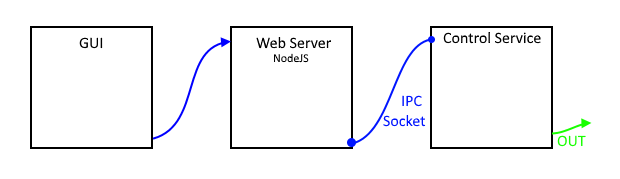
\includegraphics[width=\linewidth]{IPCDiag.png}

		\noindent \\Advantages of using sockets:
		\begin{itemize}
			\item Natively supported by any language considered for the system
			\item Efficient and fast communication
		\end{itemize}

		\noindent \\Disadvantages of using sockets:
		\begin{itemize}
			\item Bare-bones, all communication details and protocols would have to be custom written, re-inventing the HTTP wheel
			\item Would require web server to open dedicated socket connection to Control Service for every client connection
		\end{itemize}


		\subsection{Discussion}
		All three of these technologies will allow clients to communicate with the Control Service, but not all of them would meet the criteria for versatility and simplicity.
		Features will be rapidly added to the system, meaning the time spent modifying existing communication code should be minimized if possible, as it will be done often.
		Using a REST API eliminates the need for a dedicated web server by moving the client communication logic into the Control Service. It also allows changes to be made easily and rapidly, but some additional overhead is accrued in exchange for reduced development complexity.
		Using file manipulation eliminates the need for a persistent data storage system by modifying the saved disk data directly, at the expense of a speed loss.
		File manipulation also requires two code bases to be maintained for reading and writing the configuration file (web server and control service).
		Using sockets for communication is fast and efficient, but difficult to correctly implement, as very little is given automatically.
		Sockets only provide a channel for data to flow, so data transfer protocols and communication standards must be manually implemented.

		\subsection{Conclusion}
		Due to the rapid change schedule employed by this system, the ability to easily modify how data is transferred between client and server is an important factor when choosing an API technology.
		A REST API provides the most versatility and is the easiest to use out of the three options, making it the preferred choice for the Control Service API.


	\section{Control Service data storage}
		\subsection{Overview and Criteria}
		The data storage system is a crucial component of the Control Service.
		It will allow data to persist between system reboots, and serves as a backup allowing data to be copied to a new system.
		When system settings are modified, the changes travel through the Control Service, and end by modifying the LEDs.
		While setting changes are within the Control Service, they will be saved to the file system to allow user settings to persist in the frequent event of a system power loss.
		The most important aspect of data storage for this system should be maintainability.
		The constant iteration of this system will require the data's structure to be changed frequently, and possibly dramatically.
		The second most important aspect is accessibility. Reading and writing data using the system should be a simple process.
	  The third aspect is speed. The data will be stored on a device with limited processing capabilities. Saving or loading data should not be a bottleneck to system performance.

		\subsubsection{Serialization}
		Supported by most high level object oriented languages, serialization is a process by which an object is converted into a stream of bytes and then stored in a database, file, a different section of memory, or a networked device. \cite{serialization1}
		The reverse operation is called deserialization, which allows a stored file to be directly converted back into an object in memory.
		The process of serialization can be used to send object data directly from one system to another, without requiring a manual conversion routine to be written.

		\noindent \\In this system, the control flow for object serialization may look like this:

		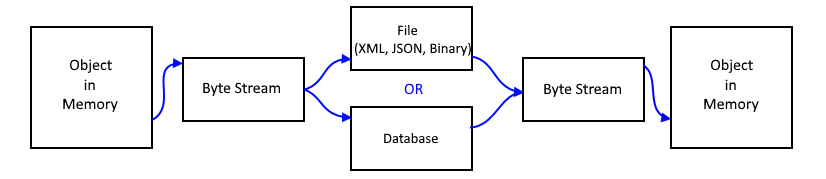
\includegraphics[width=\linewidth]{serializationDiag.png}

		\noindent \\Advantages of using serialization:
		\begin{itemize}
			\item Supported by any object oriented language considered for the project
			\item Massively simplifies saving and loading
			\item Objects can be converted directly to human readable XML, JSON, or straight to binary data
		\end{itemize}

		\noindent \\Disadvantages of using serialization:
		\begin{itemize}
			\item Loading old data after object changes have been made requires a manual conversion routine
			\item Data may take up slightly more disk space than storing raw data
		\end{itemize}


		\subsubsection{Database}
		Database are groups of highly organized data that can be easily created, retrieved, updated, and deleted. \cite{database1}
		Databases are organized into tables and rows, indexed to provide very fast and efficient data access.
		A database is typically a file or collection of files stored in a particular format that is probably not human readable.
		The data is accessed using a query language, of which there are many (SQLite, MySQL, T-SQL, SQLServer, etc).
		In typical usage, an SQL query is written and sent to an SQL service for processing and retrieval.
		The result is returned to the source that requested it.
		It is then processed row by row, where it is manually converted into a format usable by the system.

		\noindent \\In the context of this system, a database request may look like this:
		\begin{lstlisting}[language=SQL]
/* Insert new zone, ID 3, RED, 80% intensity, schedule 1 */
INSERT INTO ZONES (ID, COL, INTENS, SCHED_ID) VALUES (3, "FF0000", 0.8, 1);
/* Insert new zone, ID 4, GREEN, 40% intensity, schedule 2 */
INSERT INTO ZONES (ID, COL, INTENS, SCHED_ID) VALUES (4, "00FF00", 0.4, 2);

/* Get four columns from the zone with an id of 3 */
SELECT ID, COL, INTENS, SCHED_ID FROM ZONES WHERE ID = 3;

/* Change the color of the zone with an id of 4 to BLUE */
UPDATE ZONES SET COL = "0000FF" WHERE ID = 4;
\end{lstlisting}

		\noindent \\A loading routine that reads SQL data to produce internal objects may look like this:

	\begin{lstlisting}[language=JAVA]
Result result = SQL.executeQuery("SELECT * FROM ZONES");
while (result.next()) {
	int ID = result.getInt("ID");
	int Color = result.getInt("COL");
	float Intensity = result.getFloat("INTENS");
	Schedule WeekSchedule = Schedules.get(result.getInt("SCHED_ID"));

	Zone z = new Zone(ID, Color, Intensity, WeekSchedule);
	Zones.Add(z);
}
\end{lstlisting}

\noindent \\Advantages of using a database:
\begin{itemize}
	\item Very large amounts of data can be stored without difficulty or performance loss
	\item Storage, retrieval, and modification of data is simple and fast
	\item Data conversion can be done directly in SQL with not much difficulty
\end{itemize}

\noindent \\Disadvantages of using a database:
\begin{itemize}
	\item Separate query language required for data access
	\item Some SQL services are efficient for large amounts of data at the cost of overhead
\end{itemize}


		\subsubsection{Translation to markup}
		Internal object state can be converted into a markup configuration file and stored in plain text.
		There are several languages to choose from for markup (XML, JSON, Yaml) \cite{config1}
		A conversion function is written that takes an object and manually translates it into a format required by the chosen configuration language.
		Once the file is saved, it can be opened again and manually translated back into a memory object.

		\noindent \\In this system, the control flow for object translation to markup may look like this:

		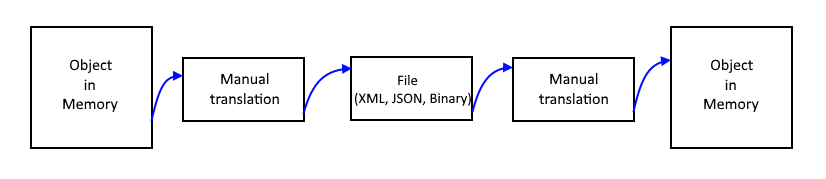
\includegraphics[width=\linewidth]{markupDiag.png}

		\noindent \\Advantages of using markup translation:
		\begin{itemize}
			\item Full control over data storage and conversion
		\end{itemize}

		\noindent \\Disadvantages of using markup translation:
		\begin{itemize}
			\item Manual translation functions (saving and loading) must be written and modified every time a change is made to any data structure
			\item Conversion of stored data from previous data format can be difficult and is required every time data changes
		\end{itemize}


		\subsection{Discussion}
		All three of these options solve the issue of persistent data storage, each has a different level of maintainability and speed.
		Serialization allows saving and loading to become trivial, nearly automatic.
		The downside is that every change to the way data is structured requires a manual translation function to be written and then thrown away.
		Using a database requires translation routines for saving and loading, but data conversion becomes simple and can be done entirely within the database.
		Serialization is easy to set up, but difficult to maintain. Databases are difficult to set up, but easy to maintain. Markup translation is difficult to set up and maintain.

		\subsection{Conclusion}
		Due to the constant iteration of the system, converting data will be a frequent and important part of the development cycle.
		That is why a database is the recommended method for the persistent storage of data.

		\section{Control Service internal state}
			\subsection{Overview and Criteria}
			The internal state of the service could be described as its short term memory.
			Input is received and processed, output to the LEDs, and then stored using long term storage if necessary.
			The internal state lets the system (and the user) know what previous input was received, without performing a time consuming long term storage retrieval.
			The system can store the current data for all LEDs, user profile settings, schedules, and any other piece of relevant information.
			That information can then be easily translated into serial data for the LEDs, file data for persistent storage, and web data for GUI display.
			The rapid iteration cycle of this system means that settings and data will change frequently and possibly dramatically.
			The internal structure of the system state should be easily modified to allow these changes to happen with little resistance.


			\subsubsection{Objects and classes}
			Object oriented programming (OOP) is a paradigm loved by some, and hated by others.
			Objects are instances of a template (\textit{class}). More or less, a class is like an ice cube tray, and objects are the resulting ice-cubes.
			An object is made up of variables (\textit{members}) and functions (\textit{behavior}).
			Objects allow complex data relationships to be expressed in real-world terms, trading some performance or memory for a simpler conceptual understanding, and a shorter development time.
			One of the most useful aspects of OOP is inheritance. Objects can inherit properties from other objects.
			For example, a \textit{Tesla Model S} is an automobile with a max speed, wheels, seats, and propulsion. But it has some additional traits such as a battery pack and autonomous driving that are not shared by every automobile.

			\noindent \\In this system, using Objects to represent internal state may look like this:

			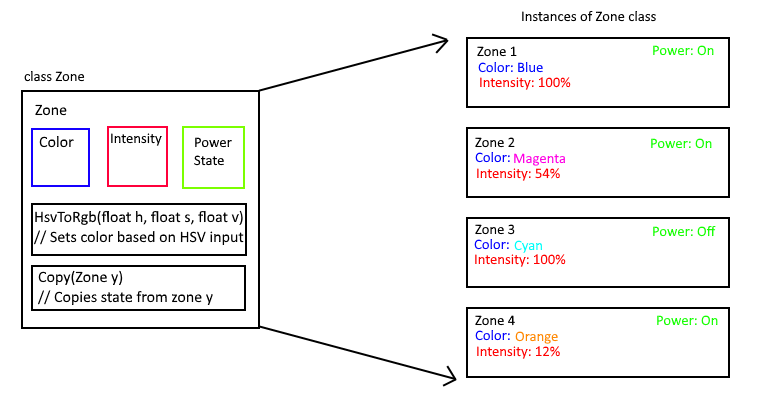
\includegraphics[width=\linewidth]{objectsDiag.png}

			\noindent \\Advantages of using objects:
			\begin{itemize}
				\item System structure and features are easily written in code, logic is organized and kept with related data
				\item Changes can be quickly and easily made
				\item Non-trivial data can be represented in an easy to understand way
			\end{itemize}

			\noindent \\Disadvantages of using objects:
			\begin{itemize}
				\item More memory is used when storing objects compared to raw integers and strings
			\end{itemize}


			\subsubsection{Structs and lists}
			Structs are a precursor to objects in many ways. They are a relic from the C programming language, but are still a useful method of representing data.
			Structures or \textit{structs} are collections of variables, usually stored consecutively in memory, which can be manipulated as singular objects, almost as if a struct is a named box in which like data can be stored.
			Structures are essentially objects without behavior. Data can be stored in a useful and organized manner, but all logic pertaining to that data must be performed in a different location.
			Lists would be used as a method of storing multiple structs of similar type (ex: zone, schedule, plant, userProfile).

			\noindent \\Advantages of using structs:
			\begin{itemize}
				\item Raw data can be organized into digestible chunks
				\item Effectively the same footprint as storing raw data
			\end{itemize}

			\noindent \\Disadvantages of using structs:
			\begin{itemize}
				\item Business logic and data kept in separate locations, making the bigger picture harder to see
			\end{itemize}


			\subsubsection{File system or database}
			This option forgoes the organization and structure provided by objects or structs, and places the system state directly into the persistent storage.
			Effectively, this method would involve the removal of short term memory in favor of immediately placing everything into long term memory.
			Using this method, the Control Service becomes an input-output machine whose purpose is to gather input from its API, read physical storage, and insert or modify existing data.
			When data is accessed using this method, the file storage is queried for the data, the data is processed, and the result is output to the LEDs.
			The Control Service would have no internal knowledge of the state of the system, instead relying on an I/O call when data is required.

			\noindent \\Advantages of using file system:
			\begin{itemize}
				\item Long term data storage is automatic
			\end{itemize}

			\noindent \\Disadvantages of using file system:
			\begin{itemize}
				\item I/O calls are expensive relative to in-memory manipulation of data
				\item Reading and writing cannot occur simultaneously, meaning the system cannot take user input while reading or writing data
				\item Processing data is difficult without a simple way to represent the data in memory
			\end{itemize}


			\subsection{Discussion}
			OOP is a modern programming paradigm used in almost all production systems where speed is not the most important factor.
			It is highly unusual for a production application to have no internal representation of data, simply because that method does not scale well for large systems.

			\subsection{Conclusion}
			Objects are a fantastic way to organize the structure of a system, as they allow the data and its relationships to be easily digested and modified.
			Logic and variables live side by side, allowing developers to practice separation of concerns.
			This project will be developed by a team of four developers, meaning that an understanding of the data structure is crucial for effective feature implementation.
			For that reason, the recommendation is to organize the system using Objects to store variable data and behavior.


		%References
		\bibliography{ref}
		\bibliographystyle{IEEEtran}

\end{document}
